\documentclass{beamer}
\usecolortheme{beaver}
\beamertemplatenavigationsymbolsempty
\setbeamertemplate{blocks}[rounded=true, shadow=true]
\setbeamertemplate{footline}[page number]
\setbeamertemplate{caption}{\raggedright\insertcaption\par}
%
\usepackage[utf8]{inputenc}
\usepackage[english, russian]{babel}
\usepackage{amssymb,amsfonts,amsmath,mathtext}
%\usepackage{subfig}
\usepackage[all]{xy} % xy package for diagrams
\usepackage{array}
\usepackage{multicol}% many columns in slide
\usepackage{hhline}%tables
\usepackage{multirow}

% Your figures are here:

\title[Классификационные ФИНН] %optional
{Классификация траекторий динамических систем с помощью физически-информированных нейросетей}


\author[Терентьев Александр] % (optional)
{Терентьев Александр Андреевич}

\institute[MIPT] % (optional)
{
  
  Московский физико-технический институт, 
  
  Физтех-школа прикладной математики и информатики\\

  Кафедра интеллектуальных систем

  Научный руководитель: к.ф.-м.н. Исаченко Р.В.
}

\date[27.06.2024] % (optional)
{27.06.2024, Москва}

% 右下角使用logo的方式
% \logo{
\includegraphics[height=1cm]{overleaf-logo}} 

%End of title page configuration block
%------------------------------------------------------------



%------------------------------------------------------------
%The next block of commands puts the table of contents at the 
%beginning of each section and highlights the current section:
%------------------------------------------------------------


\begin{document}

%The next statement creates the title page.
\frame{\titlepage}


%---------------------------------------------------------
%This block of code is for the table of contents after
%the title page
%---------------------------------------------------------


\section{}

%---------------------------------------------------------
\section{Предсказательная часть}
%---------------------------------------------------------
%Two columns

\begin{frame}
\frametitle{Классификация траекторий динамических систем}
\begin{block}{Проблема}
Существующие методы классификации многомерных рядов не используют слишком громоздкие модели и вычислительно затратны. Либо они требуют большой обучающей выборки для выделения необходимых признаков и свойств изучаемых систем. 
\end{block}
\begin{block}{Цель}
Целью работы является предложить метод для классификации многомерных временных рядов, являющимися траекториями динамических систем,  использующие априорную информацию о физической природе рядов.
\end{block}

\begin{block}{Идея}
Использовать физико-информированный подход, для классификации рядов.
\end{block}


\end{frame}

\begin{frame}
\frametitle{Постановка задачи классификации и регрессии многомерных рядов}
\begin{columns}[T] % align columns
\begin{column}{.48\textwidth}
\color{red}\rule{\linewidth}{4pt}

Задача классификации
\end{column}%
\hfill%
\begin{column}{.48\textwidth}
\color{blue}\rule{\linewidth}{4pt}

Задача регрессии
\end{column}%
\end{columns}
\begin{block}{Дано}
\begin{columns}[T] % align columns
\begin{column}{.48\textwidth}
$D = \{(X_i, y_i)\}_{i=1}^N$, где $y_i \in \overline{1, K}$ -- метка $i$-ой траектории
\end{column}%
\hfill%
\begin{column}{.48\textwidth}
$D_X = \{(\mathbf{x}_i, \mathbf{y}_i)\}_{i=1}^N$, где $\mathbf{y}_i = \ddot{\mathbf{q}}_i \in \mathbb{R}^r$ -- ускорение
\end{column}%
\end{columns}
\hfill

$X = (\mathbf{x}_1, \mathbf{x}_2,..., \mathbf{x}_T)$, 
$\mathbf{x}_i = (\mathbf{q}_i, \mathbf{\dot{q}}_i),\ \mathbf{\dot{q}}_i \in \mathbb{R}^r$ -- скорость в $i$-ый момент времени, $\mathbf{q}_i \in \mathbb{R}^r$ -- координата в $i$-ый момент времени
\end{block}
\begin{block}{Найти}
\begin{columns}[T] % align columns
\begin{column}{.48\textwidth}
$p(\hat{y}|X, D) = p(\hat{y}|L, D)p(L|X)$, где $\hat{y} \in \overline{1, K}^N$ -- предсказанные метки классов
\end{column}%
\hfill%
\begin{column}{.48\textwidth}
$p(\hat{\mathbf{y}}| \mathbf{x} , D_X)  = p(\hat{\mathbf{y}}| \mathbf{x}, L) p(L|D_X)$
$\hat{\mathbf{y}}_i = \hat{\ddot{\mathbf{q}}}_i$ -- предсказанная динамика траектории, $L \in Q$
\end{column}%
\end{columns}
\end{block}
\begin{block}{Критерий}
\begin{columns}[T] % align columns
\begin{column}{.48\textwidth}
Метрики Accuracy и F1Macro 
\end{column}%
\hfill%
\begin{column}{.48\textwidth}

$\mathcal{L}(\hat{\mathbf{y}}, \mathbf{y})  = \frac{1}{T}\sum_{i=1}^{T} \| \mathbf{\hat{y}}_i - \mathbf{y}_i \|_2^2$
\end{column}%
\end{columns}
\end{block}
\end{frame}


\begin{frame}
\frametitle{Лагарнжева нейронная сеть}

\begin{figure}[H]
\centerline{
    \xymatrix{
    \mathbf{x}_i = (\mathbf{q}_i, \dot{\mathbf{q}}_i) \ar@{->}[rrr]^-{\hat{L} \colon (\mathbf{x} | \mathbf{w}) \to L_\mathbf{x}} & & & L_\mathbf{x} \ar@{->}[r]^-{\nabla L} & \frac{d}{d t} \frac{\partial L}{\partial \dot{\mathbf{q}}} =\frac{\partial L}{\partial \mathbf{q}} \ar@{->}[rr]^-{{\ddot{\mathbf{q}}_i = g\left(\mathbf{q}_i, \dot{\mathbf{q}}_i\right)}} &  & \mathbf{y}_i = \ddot{\mathbf{q}}_i
    }
}
\caption{Схема нейронной сети}
\label{fig: LNN}
\end{figure}
\begin{block}{Параметризация}
\begin{enumerate}
\item$p(L|D),\ L \in Q = \{\hat{L} \colon (\mathbf{x} | \mathbf{w}) \to L_{\mathbf{x}, \mathbf{w}}\}$
$\hat{L}$ - полносвязная нейронная сеть с функцией активации SoftPlus, $w$ - параметры нейронной сети.
\item $p(L|D) = [L = \hat{L}]$, где $\hat{L}$ ~-- ОМП лагранжиана системы, полученная из $\mathcal{L}(\hat{\mathbf{y}}, \mathbf{y}) \to min$
\end{enumerate}
\end{block}

\begin{block}{Система для нахождения ускорений}
\[
p(\hat{y}| X, L): \left(\nabla_{\dot{\mathbf{q}} \dot{\mathbf{q}}} L\right)\ddot{\mathbf{q}} = \left[\nabla_{q} L-\left(\nabla_{\dot{\mathbf{q}}\mathbf{q}} L\right) \dot{\mathbf{q}}\right].
\]
\end{block}

\end{frame}



%---------------------------------------------------------
\begin{frame}
\frametitle{Модификация функции потерь с регуляризацией}
В исходной архитектуре сети в каждой точки траектории решается СЛАУ. Проблема в том, что у матрицы $\mathbf{H}_L(\mathbf{q}, \dot{\mathbf{q}}) = \nabla_{\dot{\mathbf{q}} \dot{\mathbf{q}}} L$ собственные значения могут быть сколь угодно маленькими. 

 \[\mathbf{H}\hat{\ddot{\mathbf{q}}} = \hat{\mathbf{b}} \equiv \nabla_{q} L-\left(\nabla_{\dot{\mathbf{q}}\mathbf{q}} L\right) \dot{\mathbf{q}}, \]

$$
\hat{\ddot{\mathbf{q}}} = \mathbf{H}^{-1}\left[\nabla_{q} L-\left(\nabla_{\dot{\mathbf{q}}\mathbf{q}} L\right) \dot{\mathbf{q}}\right],
$$

$$
\mathbf{H}\ddot{\mathbf{q}} \equiv \mathbf{b}.
$$
Тогда изменим функцию потерь так, чтобы штрафовать за собственные значения матрицы $H$  меньше 1, а вместо разности ускорений возьмем невязку для полученной СЛАУ

$$
 \mathcal{L}^{\text{mod}}(\textbf{w}) = \frac{1}{T}\sum_{i=1}^{T} \| \mathbf{\hat{b}}_i - \mathbf{b}_i \|_2^2  + \alpha \text{act}(\beta (\lambda(H_{\ddot{q}}) - 1)).
$$
\end{frame}

\begin{frame}
\frametitle{Идея классификатора}
$$A(L) = \nabla_{q} L-\left(\nabla_{\dot{\mathbf{q}}\mathbf{q}} L\right) \dot{\mathbf{q}}, H(L) = \nabla_{\dot{\mathbf{q}} \dot{\mathbf{q}}} L$$

\begin{figure}
\centering
\xymatrix{
X  \ar@{->}[r]^-{\text{LNN}}  & \hat{L}=g(x|w) \ar@{->}[rr]^{{L_N^{i} = A(L)\left(\mathbf{q}_i, \dot{\mathbf{q}}_i\right)}} & {} & L_N \in \mathbb{R}^N \ar@{->}[rrr]^-{\text{classifier}: R^N \to K} &  &  & \hat{y} \\
 & Q_N \sim U([-L, L]^{2r}) \ar@{->}[ur]  &  &  &  &  &  &
}
\caption{Схема нейронной сети}
\label{fig: LNN}
\end{figure}
\begin{block}{Аппроксимация нормы}

$$\overline{|A(L)\left(\mathbf{q}, \dot{\mathbf{q}}\right)|^2 + \|H(L)\left(\mathbf{q}, \dot{\mathbf{q}}\right)\|_2^2}$$
$$\|H(L)\left(\mathbf{q}, \dot{\mathbf{q}}\right)\|_2^2 \approx \text{const}$$
\end{block}

\end{frame}

\section{Теоретические результаты}

\begin{frame}
\frametitle{Эквивалентность приближенной задачи исходной}
Было показано, что приближение исходных лагранжианов систем через их оценки не портит отделимость классов систем.
\begin{block} {Теорема (Терентьев, 2024)}
Пусть есть конечное семейство непересекающихся замкнутых выпуклых множеств $\mathcal{A}$ в нормированном пространстве $\mathbb{L}$, тогда существует $\epsilon > 0$, что для любого преобразования пространства $\phi$ такое, что $\|\phi(\mathcal{A}_{i}) - \mathcal{A}_{i}\| < \epsilon$ множества из семейства $\phi{\mathcal{A}}$ попарно сильно отделимы.
\end{block} 
\end{frame}

\begin{frame}
\frametitle{Эквивалентность нахождения минимума невязки и отклонения ускорений}
\begin{block} {Норма в пространстве лагранжианов}
\[
p(\hat{y}| X, L): \left(\nabla_{\dot{\mathbf{q}} \dot{\mathbf{q}}} L\right)\ddot{\mathbf{q}} = \left[\nabla_{q} L-\left(\nabla_{\dot{\mathbf{q}}\mathbf{q}} L\right) \dot{\mathbf{q}}\right].
\]
$$A(L) = \nabla_{q} L-\left(\nabla_{\dot{\mathbf{q}}\mathbf{q}} L\right) \dot{\mathbf{q}}, \mathbf{H}(L) = \nabla_{\dot{\mathbf{q}} \dot{\mathbf{q}}} L,$$
$$\|L\|_L = \|(A(L), \mathbf{H}(L))\|_2,$$
\begin{equation}\label{eq:linear_equation_acc}
A(L)(\mathbf{q}, \dot{\mathbf{q}}) = H(L)(\mathbf{q}, \dot{\mathbf{q}})\ddot{\mathbf{q}}.
\end{equation}
\end{block}

\begin{block} {Теорема (Терентьев, 2024)}
$\|\delta L\|_L = 0 \Leftrightarrow \text{п.в.}~\delta \ddot{q} = 0$, где $\delta L = L' - L, ~\delta \ddot{q} = \ddot{q}' - \ddot{q}, ~\text{где} \ L',\ L \in \mathcal {X}$ являются вариациями лагранжиана и ускорения на множестве ~$\mathcal {X}$, на котором функциональное уравнение \ref{eq:linear_equation_acc} относительно $L$ имеет единственное решение, и $\forall L\in \mathcal{X}:~\mathbf{H}(L) \not\equiv 0, $.
\end{block}

\end{frame}



\begin{frame}
\frametitle{Эквивалентность исходной оптимизационной задачи и задачи с ограничениями}

Было доказано, что выбранные ограничение на множество искомых функций не уменьшает общность задачи нахождения динамики. Рассматривается следующая функция потерь
$$
 \mathcal{L}^{mod}(\textbf{w}) = \frac{1}{T}\sum_{i=1}^{T} \| \mathbf{\hat{b}}_i - \mathbf{b}_i \|_2^2  + \alpha \text{act}(\beta (\lambda(H_{\ddot{q}}) - 1)).
$$

\begin{block} {Теорема (Терентьев, 2024)}
Если лагранжианы заданы на компакте, то существуют неотрицательные числа $a, b$ такие, что $det H \ge a$, а собственные значения матрицы $H$ не меньше $b$
\end{block} 
\end{frame}

\begin{frame}
\frametitle{Аппроксимация нормы}
Исходное пространство бесконечномерное. Для задачи классификации требуется спроецировать его на евклидово пространство. Рассмотрим норму
$$A(L) = \nabla_{q} L-\left(\nabla_{\dot{\mathbf{q}}\mathbf{q}} L\right) \dot{\mathbf{q}}, H(L) = \nabla_{\dot{\mathbf{q}} \dot{\mathbf{q}}} L,$$
$$\|L\|_L = \|(A(L), H(L))\|_2,$$
\begin{equation*}
A(L)(\mathbf{q}, \dot{\mathbf{q}}) = H(L)(\mathbf{q}, \dot{\mathbf{q}})\ddot{\mathbf{q}}.
\end{equation*}

\begin{block} {Теорема (Терентьев, 2024)}
Исходная норма $\|\cdot\|_L$ с любой наперед заданной точностью $\epsilon$ приближается $l_2$-нормой, при стремлении числа сэмплов $N$ и меры пространства из которого берут сэмплы $\Omega$ к бесконечности
\[
\begin{split}
    \|(A(L),  H(L))\|_2 = \sqrt{\int |A(L)\left(\mathbf{q}, \dot{\mathbf{q}}\right)|^2 + \|H(L)\left(\mathbf{q}, \dot{\mathbf{q}}\right)\|_2^2  d\Omega} \approx
\\
\mu(\Omega) \cdot \overline{|A(L)\left(\mathbf{q}, \dot{\mathbf{q}}\right)|^2 + \|H(L)\left(\mathbf{q}, \dot{\mathbf{q}}\right)\|_2^2}
\end{split}
\]
\end{block} 
\end{frame}

\begin{frame}
\frametitle{Остатки траектории в зависимоти от регуляризации}

Использовался синтетический набор данных для траекторий двойного маятника. Из графика остатков следует, что без регуляризации получается неинформативное предсказание динамики.

\begin{figure}[H]
 \centering
 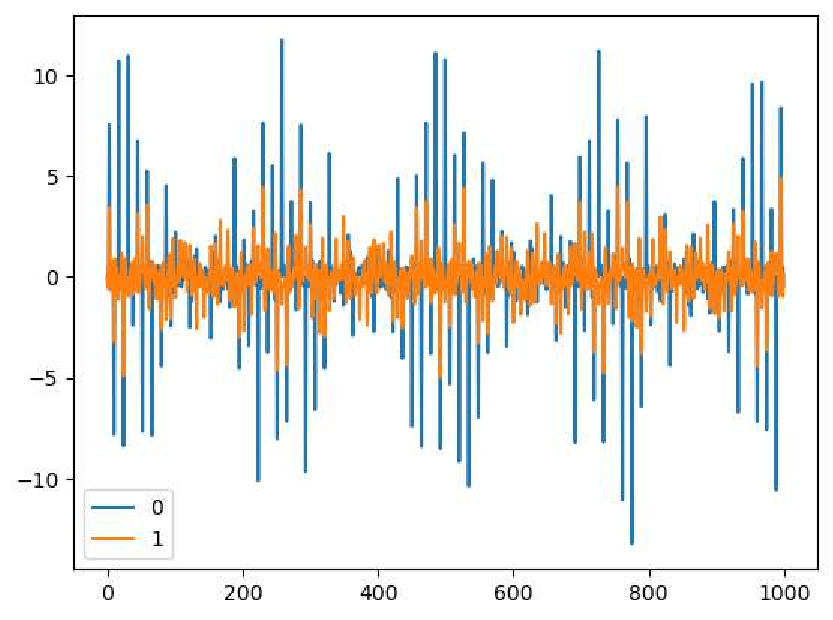
\includegraphics[scale = 0.37]{output_resid_5.pdf}
 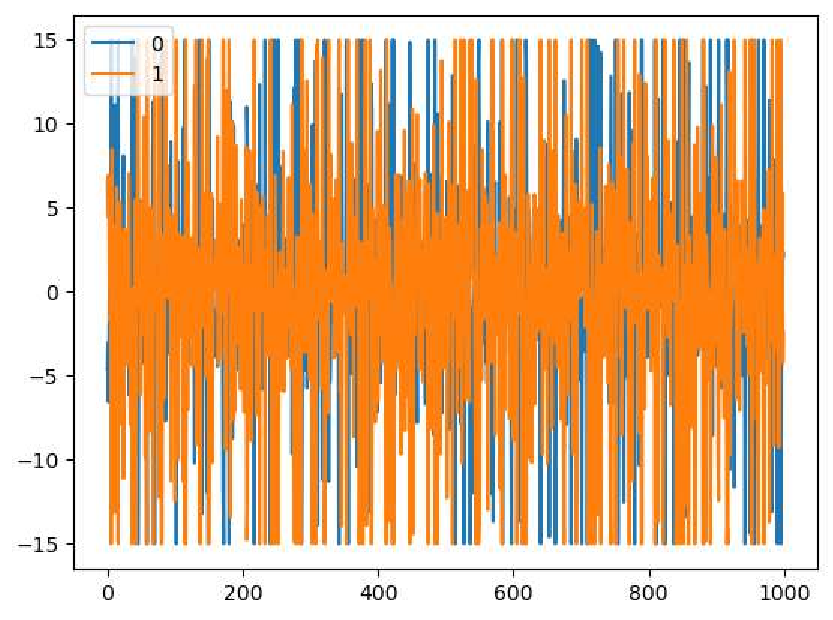
\includegraphics[scale = 0.37]{output_resid_0.pdf}
 \caption{График остатков для траектории двойного маятника, слева с регуляризацией, справа без}
 \label{fig: trajectory3}
\end{figure}

\end{frame}

\begin{frame}
\frametitle{Вычислительный эксперимент}
Исследования проводились на наборе данных Physical Activity Monitoring(PAMAP2)
\begin{enumerate}
    \item Записи с трех наборов гироскопов и акселерометров: закрепленных на запястье преобладающей руки, закрепленных на груди, закрепленных на локте преобладающей руки
    \item Число испытуемых: $M = 9$
    \item Число видов активностей(классов): $K = 24$
    \item Каждая активность длилась 2-4 минуты
    \item Частота сэмплирования 100 Гц
\end{enumerate}

\end{frame}

\begin{frame}
\frametitle{Восстановление динамики системы}
\begin{figure}[H]
     \centering
     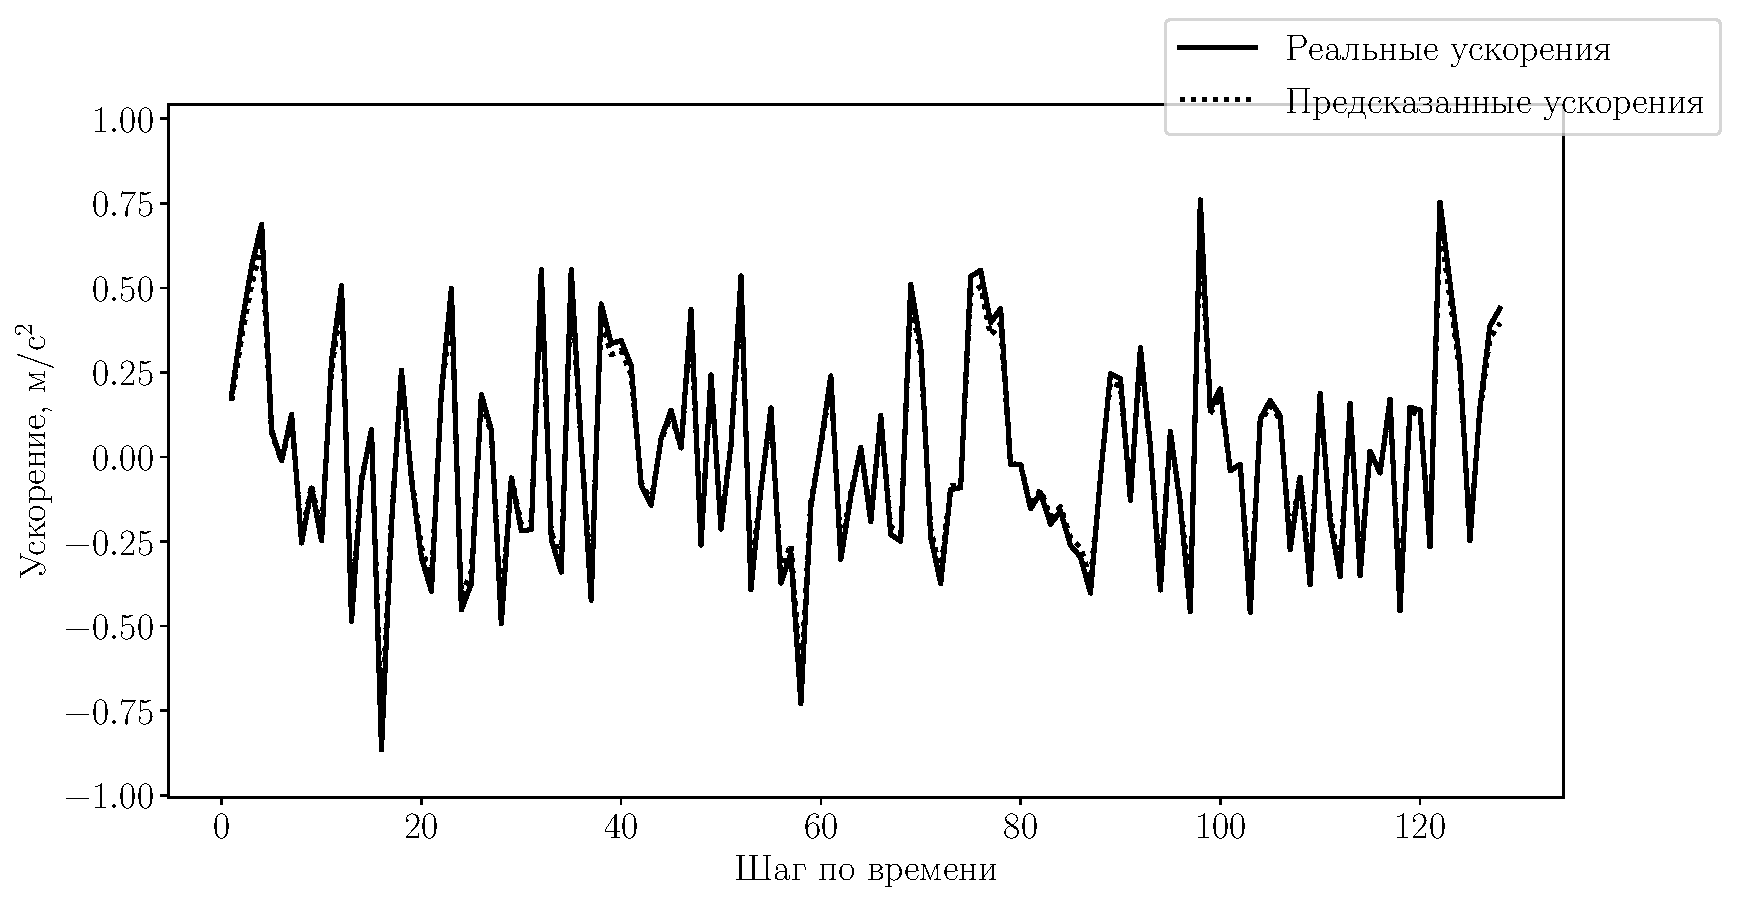
\includegraphics[width = 0.5\textwidth]{experiment4_1000.pickle_results_a.pdf}%
     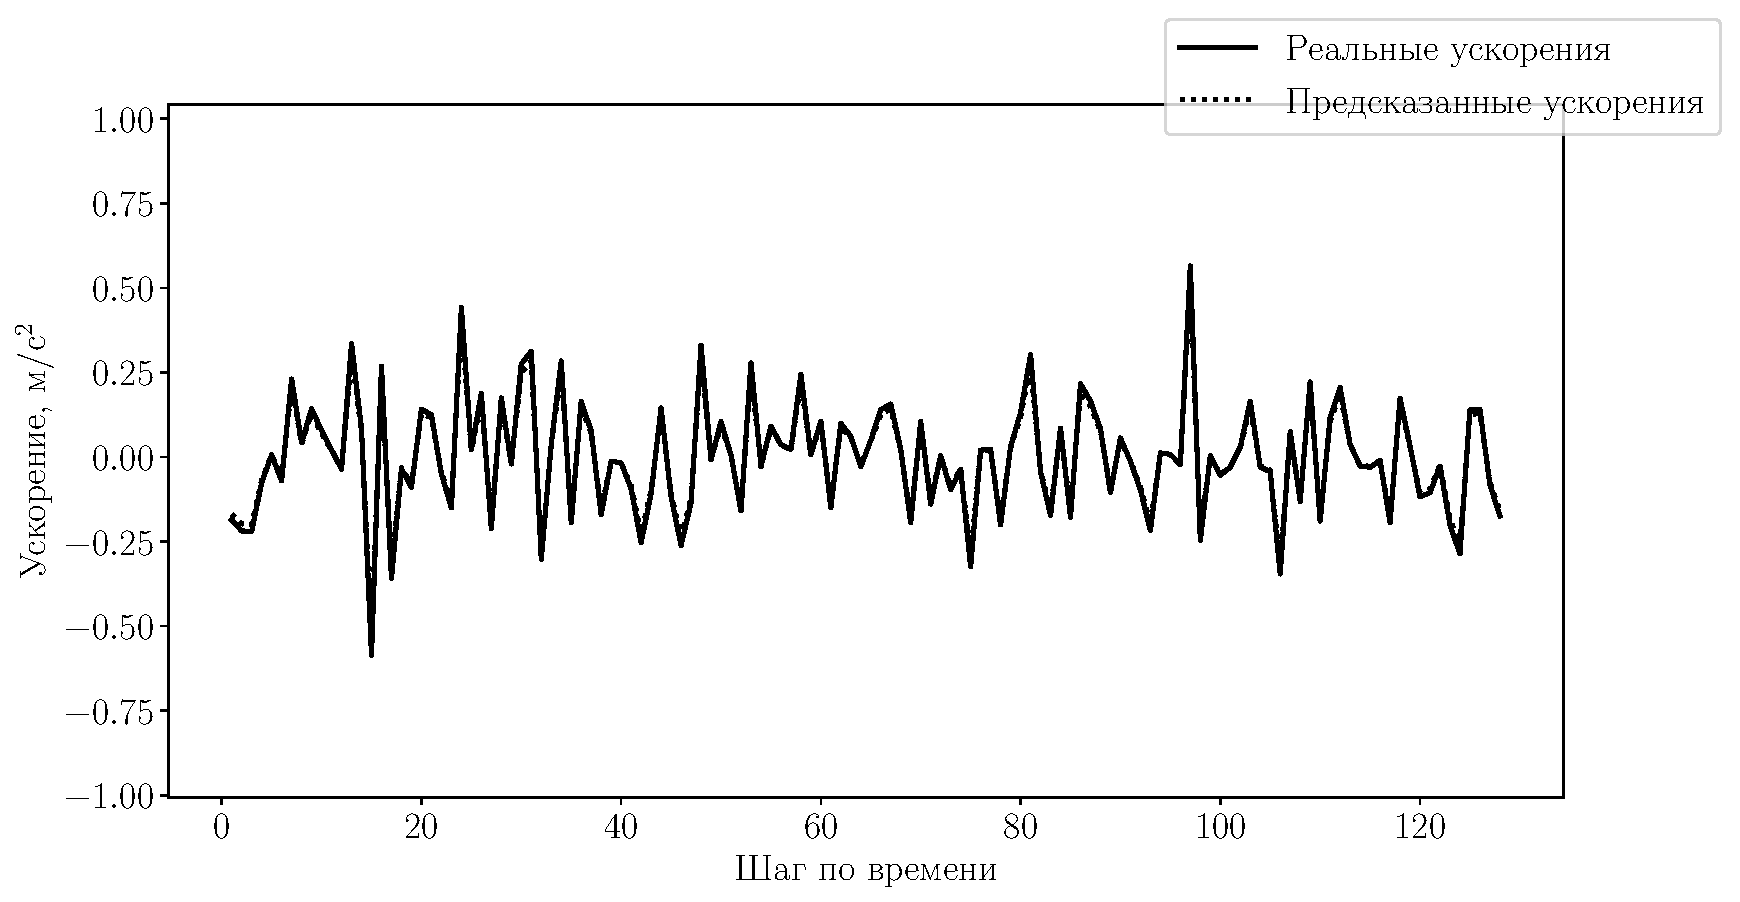
\includegraphics[width = 0.5\textwidth]{experiment4_1000.pickle_results_b.pdf}
     \caption{Временной ряд зависимости ускорения от времени для тестовой выборки}
     \label{fig: trajectory}
\end{figure}
\begin{enumerate}
    \item Из полученных графиков следует, что точность восстановления динамики системы, требуемая для задачи классификации, достается.
    \item Нефизические осцилляции отсутствуют
\end{enumerate}
\end{frame}

  

\begin{frame}
\frametitle{Распределение классов в пространстве Лагранжианов}
\begin{figure}[H]
 \centering
 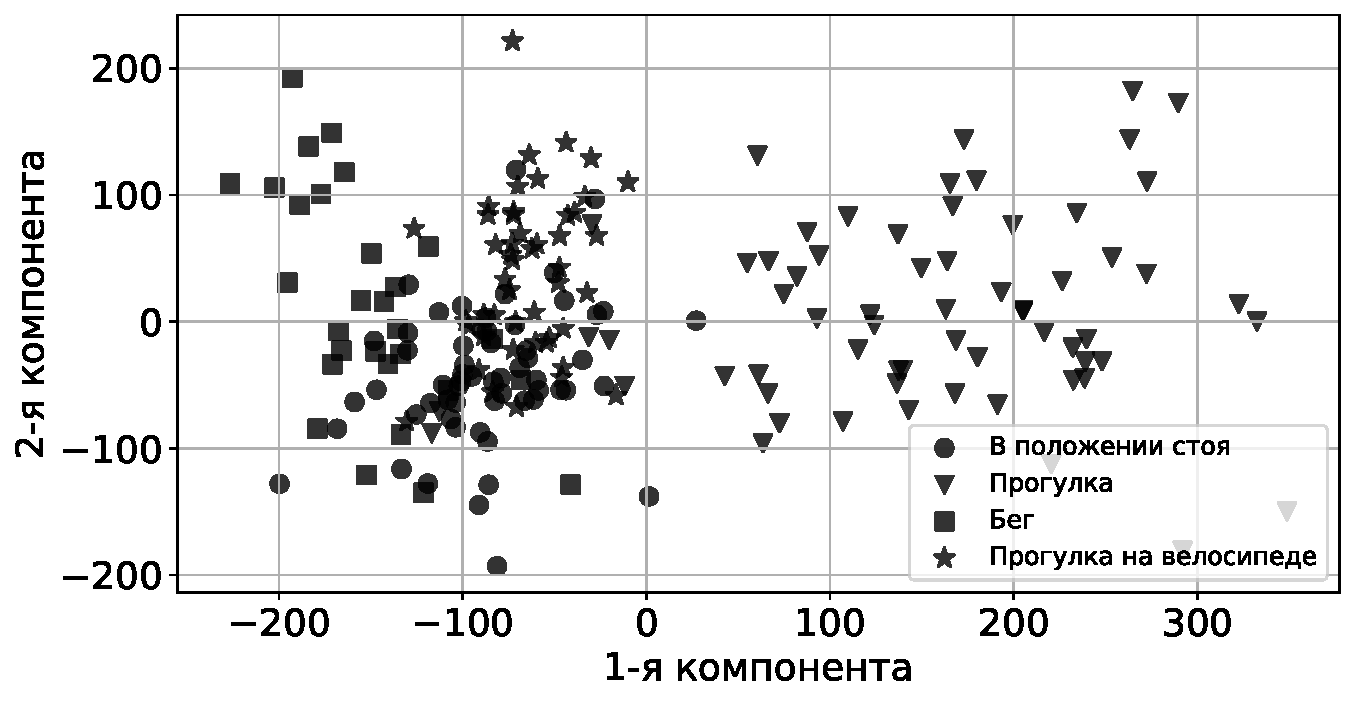
\includegraphics[scale = 0.45]{Data.pdf}
 \caption{Проекция пространства лагранжианов на плоскость}
 \label{fig: 2D}
\end{figure}

\end{frame}

\begin{frame}
\frametitle{Сравнение качества работы классификаторов}
\begin{figure}[H]
 \centering
 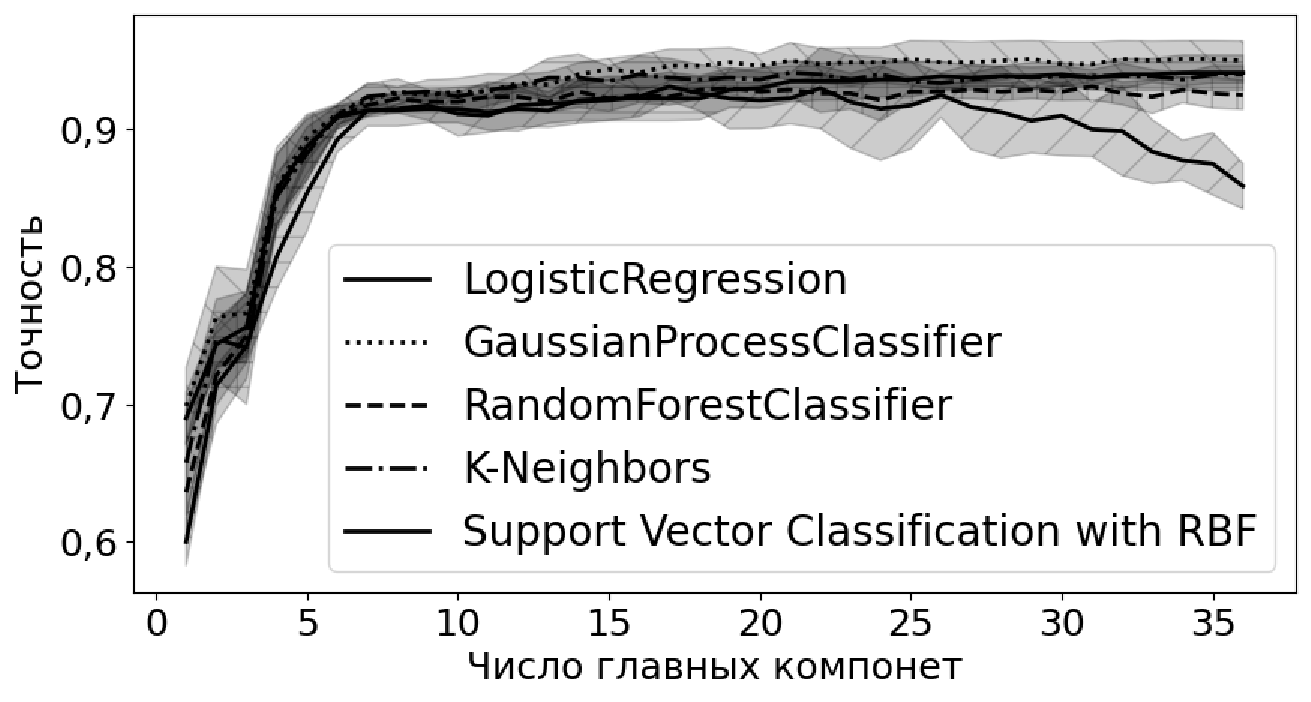
\includegraphics[scale = 0.4]{Accuracy.pdf}
 \caption{Точность классификации выбранных методов в зависимости от количества главных компонент}
\end{figure}


\end{frame}

\begin{frame}
\frametitle{Сравнение качества работы классификаторов}
\begin{table}[H]
    \centering
    \resizebox{\textwidth}{!}{\begin{tabular}{|l|lll|}
    \hline
    \multicolumn{1}{|c|}{\multirow{2}{*}{Классификатор}} & \multicolumn{3}{c|}{Метрика}                                                                     \\ \cline{2-4} 
    \multicolumn{1}{|c|}{}                               & \multicolumn{1}{l|}{Accuracy}         & \multicolumn{1}{l|}{Balanced-accuracy} & F1 Macro        \\ \hline
    Логистическая регрессия                              & \multicolumn{1}{l|}{$0,927 \pm  0.014$} & \multicolumn{1}{l|}{$0,924 \pm 0,13$}    & $0,927 \pm 0,14$  \\ \hline
    \textbf{Гауссовский процесс}                                  & \multicolumn{1}{l|}{$\mathbf{0,946} \pm \mathbf{0,010}$}  & \multicolumn{1}{l|}{$\mathbf{0,941} \pm \mathbf{0,011}$}   & $\mathbf{0,946} \pm \mathbf{0,010}$ \\ \hline
    Случайный лес                                        & \multicolumn{1}{l|}{$0,932 \pm 0,007$}  & \multicolumn{1}{l|}{$0,928 \pm 0,008$}   & $0,933 \pm 0,008$ \\ \hline
    K-ближайших соседей                                  & \multicolumn{1}{l|}{$0,939 \pm 0,009$}  & \multicolumn{1}{l|}{$0,935 \pm 0,010$}   & $0,940 \pm 0,008$ \\ \hline
    SVC с гауссовским ядром                              & \multicolumn{1}{l|}{$0,933 \pm 0,012$}  & \multicolumn{1}{l|}{$0,927 \pm 0,01$3}   & $0,933 \pm 0,011$ \\ \hline
    \end{tabular}}
    \caption{Точность классификации на предложенной векторизации данных}
\end{table}
\begin{enumerate}
    \item Линейные классификаторы лучше справляются с классификацией, меньше переобучаются
    \item Среди линейных классификаторов лучше всего себя показывает гауссовский процесс
    \item Логистическая регрессия имеет тенденцию к переобучению
\end{enumerate}
\end{frame}

\begin{frame}
\frametitle{Выносится на защиту}

\begin{enumerate}
    \item Предложен метод физико-информированного подхода к классификации многомерных временных рядов, на основе классификации систем их порождающие.
    \item Доказано, что выбранная векторизация сохраняет отделимость классов.
    \item Доказано, что выбранная проекция пространства лагранжианов приближает норму с любой наперед заданной точностью и эквивалентность нахождения минимума невязки и отклонения ускорений и условия для этого.
    \item Исследованы методы метрической классификации в данном пространстве и показано, что линейные классификаторы дают лучшие метрики классификации. 
\end{enumerate}
\end{frame}


\end{document}